\section{Nome do Jogo}
Colocar duas referencias
Ogof e o templo das joias.

\section{\textit{High Concept} do Jogo}
Ogof e o templo das joias é um game de fantasia, em que o jogador assumirá o papel de 3 diferentes figuras, e trabalhar em conjunto para progredir.
% Ogof e o templo das joias é um game de fantasia, exploração e puzzle em que você irá assumir o papel de 3 figuras de diferentes épocas do tempo, 
% % cada qual com suas forças e fraquezas, para progredir será necessário explorar as forças de cada personagem
% e trabalhar em conjunto para descobrir os planos de Ogof.

% Conceito em 150 caracteres


\section{Gênero}

O jogo será 3D em terceira pessoa, com fases que irão misturar diversas mecânicas como \textbf{puzzle, hack em slash} e exploração. Cada fase será linear com a dificuldade gradualmente aumentada até o final da fase, em que cada uma terá um miniboss.

% Descreva e justifique o genero do jogo

\section{Púbico Alvo}

Descreva e justifique o publico alvo do jogo
Adolescentes a partir de 16 anos....
\vfill
\pagebreak

\section{\textit{Game Flow}}
\begin{figure}[htb]
	\caption{\label{fig_grafico}Fluxo de telas}
	\begin{center}
	    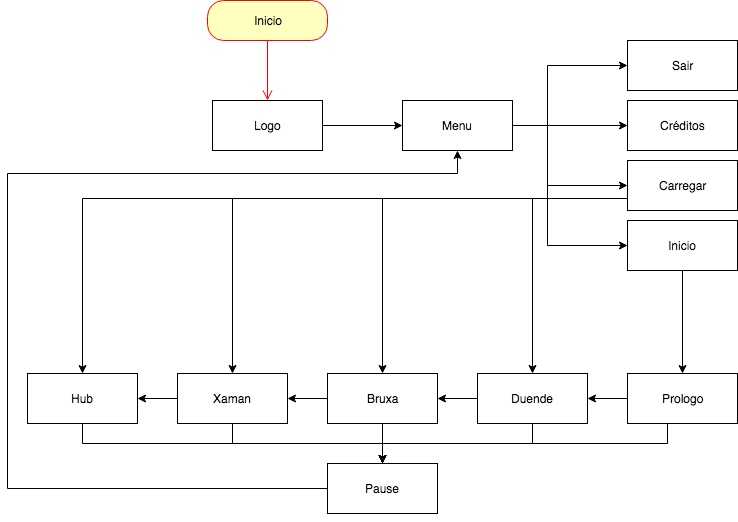
\includegraphics[width=\textwidth]{imagens/Flow.png}
	\end{center}
	\legend{Fonte: Própria Autoria}
\end{figure}
Ilustração ou tabela que demonstre todas as telas que o jogo terá e como se relacionam entre si

\section{Estilo estético}

cartoon Resumo
Colocar fontes, bibliografia colocar capa do livro/imagem referencia

\section{Inspirações}
\subsection{Outlander}
Em 1945, em lua de mel na Escócia, a enfermeira em combate Claire Randall é misteriosamente transportada através do tempo para o ano de 1743.

\subsection{Filha de Feiticeira}
Este romance de Celia Rees narra, em forma de diário, a história de Mary Nuttall, uma adolescente inglesa do século XVII que se vê obrigada a fugir para a América para não ter o mesmo destino de sua avó, condenada à forca sob acusação de feitiçaria.

\subsection{Desencanto}
Bean é uma princesa que vive no reino mágico de Dreamland ao lado de Luci, seu demônio pessoal, e de Elfo, seu melhor amigo que a acompanham em sua jornada de alcoolismo, brigas de bar e descobertas inusitadas.

\subsection{Os Vingadores - Guerra infinita}
Inspirou a proposta de coleta de joias e a personalidade de Ogof teve referência no personagem Thanos.

\subsection{Franquia God of War}

\begin{figure}[htb]
	\caption{\label{god_of_war}God of War}
	\begin{center}
	    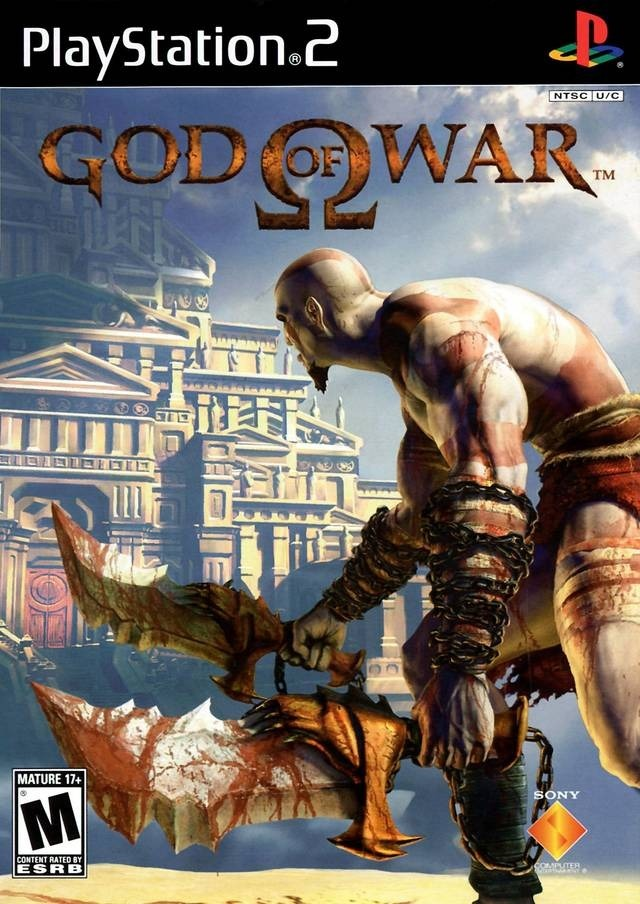
\includegraphics[width=\textwidth/2]{imagens/GodofWar.jpg}
	\end{center}
	\legend{SIE Santa Monica Studio - 2005 à 2018}
\end{figure}
Sinopse:

Inspirou a animação, técnica de câmera e combate do gameplay.

\subsection{Sonhos de uma noite de verão}

\begin{figure}[htb]
	\caption{\label{sonhos_shakespeare} Capa Sonhos de uma noite de Verão}
	\begin{center}
	    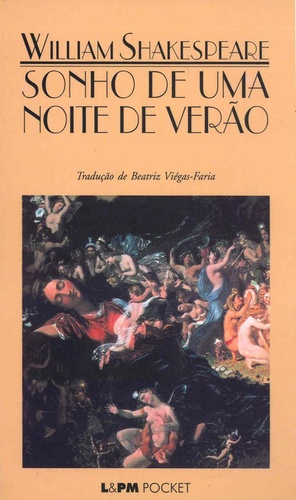
\includegraphics[width=\textwidth/2]{imagens/Sonhos.jpg}
	\end{center}
	\legend{L\&PM Pocket, William Shakespeare - 1605}
\end{figure}


Sinopse:

\subsection{Brownies}

\begin{figure}[htb]
	\caption{\label{fig_grafico}\textbf{Brownie} por Arthur Rackham }
	\begin{center}
	    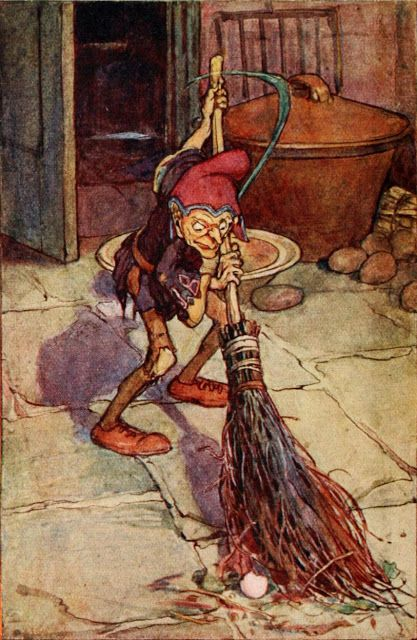
\includegraphics[width=\textwidth/2]{imagens/brownie.jpg}
		\end{center}
	\legend{William Shakespeare - 1605}
\end{figure}

Brownies são pequenos seres noturnos do folclore britânico, que cuidam dos afazeres da casa, se ofendem facilmente e evitam serem vistos pelos humanos \cite{britannica_2011}, traços de personalidades que utilizamos como inspiração para a formulação do Duende.
Todo: Inserir as referências na bibliografia, estou tendo dificuldades para achar os livros no formato digital.

\vfill
\pagebreak


\subsection{Alux}
\begin{figure}[htb]
	\caption{\label{fig_grafico}Alux}
	\begin{center}
	    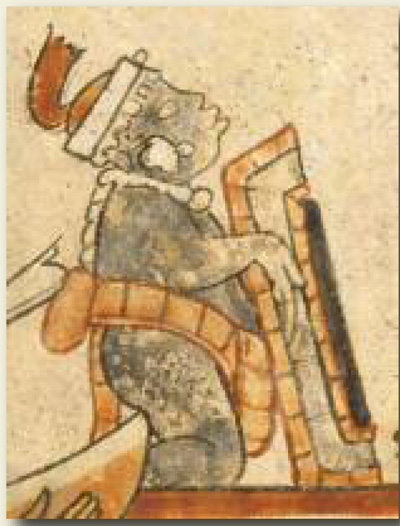
\includegraphics[width=\textwidth/2]{imagens/alux.jpg}
	\end{center}
	\legend{Fonte: \citeonline{judith_2009}}
\end{figure}

Alux são pequenas criaturas da mitologia de alguns povos Maias, costumeiramente são invisíveis, mas podem se tornar visíveis para se comunicar e assutar humanos.  São responsáveis pela boa colheita, espantando animais e controlando a chuva \cite{judith_2009}. 

\vfill
\pagebreak

\subsection{Siempre Bruja}

\begin{figure}[htb]
	\caption{\label{siempre}Siempre Bruja}
	\begin{center}
	    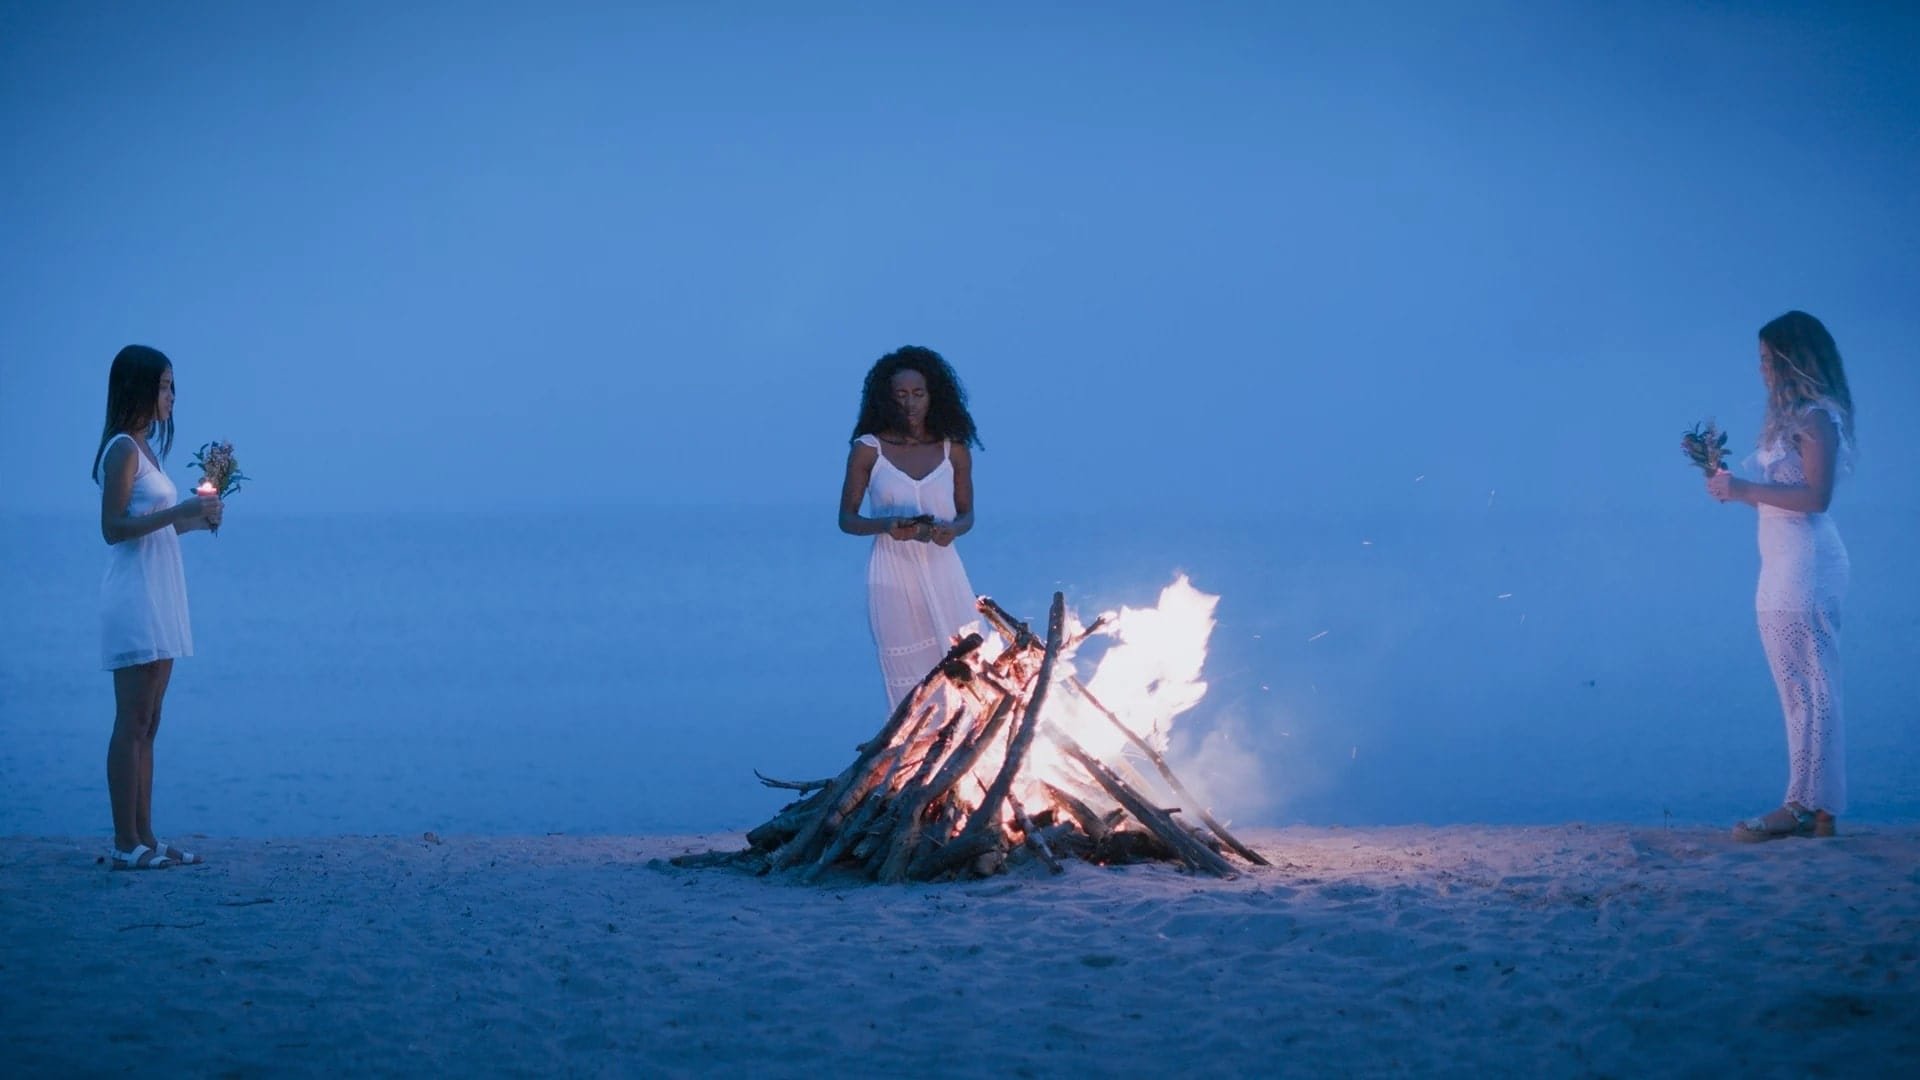
\includegraphics[width=\textwidth]{imagens/SiempreBruja.jpg}
	\end{center}
	\legend{Fonte: \citeonline{judith_2009}}
\end{figure}

A série que conta a história de uma bruxa negra e escrava que é transportada  pelo tempo para enfrentar um grande bruxo inspirou os poderes da bruxa e itens com os quais trabalha. 

\vfill
\pagebreak

\section{Equipe de Desenvolvimento}
Tabelar
A equipe dividiu-se de forma a otimizar as forças de cada um dos integrantes, desta forma ficamos com a seguinte divisão de tarefas não rígidas:

Marina atuou fortemente com o game design, character design e história. 

Pedro atuou como programador e game design

Eric atuou como arte técnica, animação e programação